\documentclass{article}
\usepackage{forest}
\usetikzlibrary{arrows.meta}
\begin{document}

\begin{figure}[h]
\centering
\begin{forest}
  for tree={circle, draw, minimum size=2em, inner sep=1pt, l sep=1.5em, s sep=1em, edge={-Stealth}},
  forked edges
  [8, fill=blue!20
    [3, fill=red!20 [3] [12] [8]]
    [2, fill=red!20 [2] [4] [6]]
    [8, fill=red!20 [14] [5] [8]]
  ]
\end{forest}
\caption{A two-ply game tree with forked edges.}
\end{figure}

\begin{figure}[h]
\centering
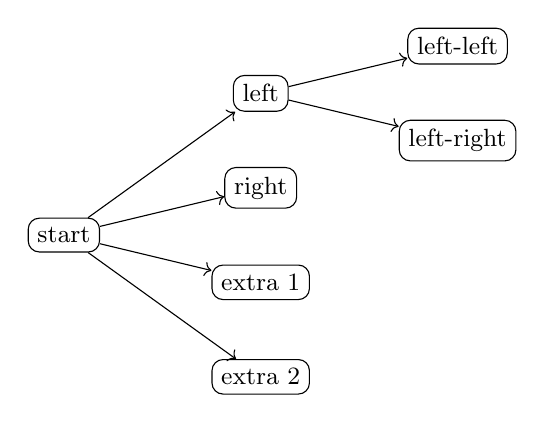
\begin{tikzpicture}[grow'=right, level distance=2.5cm, sibling distance=1.2cm,
  every node/.style={draw, rounded corners, font=\small},
  edge from parent/.style={draw, ->}]
\node {start}
  child {node {left}
    child {node {left-left}}
    child {node {left-right}}}
  child {node {right}}
  child foreach \x in {1,2} {node {extra \x}};
\end{tikzpicture}
\caption{A tree growing to the right with \texttt{child foreach}.}
\end{figure}

\end{document}
